\section{High-order accurate modified equation schemes} \label{sec:highOrderModifiedEquationSchemes}

In this section we consider efficient approaches to implement high-order accurate
modified equation schemes on Cartesian and curvilinear grids.

The modified equation schemes are based on the Taylor series expansion $\Dpt\Dmt u$,
\ba
  \Dpt\Dmt u & = \p_t^2 u + 2 \f{\dt^2}{4!} \p_t^4 u + 2 \f{\dt^4}{6!} \p_t^6 u + \ldots \\
      & = \sum_{m=1}^\infty  2 \f{\dt^{2(m-1)}}{(2m)!} \p_t^{2m} u 
\ea
Using $\p_t^2 u = c^2\Delta u$ and discretizing in space leads to the modified equation scheme
\ba
  \Dpt\Dmt u_\jv & = c^2 \Delta_{h} u_\jv + 2 \f{\dt^2}{4!} (c^2 \Delta)_h^2 u_\jv + 2 \f{\dt^4}{6!} (c^2 \Delta)_h^3 u_\jv + \ldots \\
      & = \sum_{m=1}^{p/2}  2 \f{\dt^{2(m-1)}}{(2m)!} (c^2 \Delta)_h^m u_\jv
\ea
There are $p/2$ terms on the right-hand-side, for example, an eighth-order accurate scheme is 
\ba
  \Dpt\Dmt u_\jv & = c^2 \Delta_{h,8} u_\jv 
           + \f{\dt^2}{12}     (c^2 \Delta)^2_{h,6}  u_\jv
           + \f{\dt^4}{360}    (c^2 \Delta)^3_{h,4}  u_\jv 
           + \f{\dt^6}{20,160} (c^2 \Delta)^4_{h,2}  u_\jv 
\ea
where, for example, $(c^2 \Delta)^3_{h,4}$ denotes a fourth-order accurate approximation to $(c^2 \Delta)^3$.

High-order accurate central difference approximations to spatial derivatives of different orders can be written in the form
of the following expansions in powers of $\Dpx\Dmx$, 
% \ba
%    \p_x u   &= \Dzx     \left[ \sum_{\mu=0}^\infty   \beta_\mu^{(1)} (-\dx^2 \Dpx\Dmx)^\mu  \right] u_\jv , \\
%    \p_x^2 u &= \Dpx\Dmx \left[ \sum_{\mu=0}^\infty   \beta_\mu^{(2)} (-\dx^2 \Dpx\Dmx)^\mu  \right] u_\jv , \\
%    \p_x^3 u   &= \Dzx\Dpx\Dmx   \left[ \sum_{\mu=0}^\infty   \beta_\mu^{(3)} (-\dx^2 \Dpx\Dmx)^\mu  \right] u_\jv , \\
%    \p_x^4 u &= (\Dpx\Dmx)^2 \left[ \sum_{\mu=0}^\infty   \beta_\mu^{(4)} (-\dx^2 \Dpx\Dmx)^\mu  \right] u_\jv .
% \ea 
% In general, odd and even derivatives have the expansions
\bat
   \p_x^{2m+1} u   &= \Dzx(\Dpx\Dmx)^m   \left[ \sum_{\mu=0}^\infty   \beta_\mu^{(2m+1)} (-\dx^2 \Dpx\Dmx)^\mu  \right] u_\jv , &&\quad m=0,1,2,3,\ldots\\
   \p_x^{2m} u &= (\Dpx\Dmx)^m \left[ \sum_{\mu=0}^\infty   \beta_\mu^{(2m)} (-\dx^2 \Dpx\Dmx)^\mu  \right] u_\jv             , &&\quad m=1,2,3,\ldots
\eat
The coefficients $\beta_\mu^{(\nu)}$ can be found by Taylor series. A nice trick is to substitute $u= e^{i kx}$ and $u_\jv = e^{i k j \dx}$
into the expansions and equate powers of $\xi = k\dx$. To do this we use the Fourier symbols
\ba
  \p_x e^{ikx}            & = i k ~ e^{ikx}, \\
  \p_x^2 e^{ikx}          & = -k^2 ~ e^{ikx}, \\
  \Dzx  e^{i k j \dx}     &= \f{i\sin(\xi)}{\dx} ~e^{i k j \dx} , \\
  \Dpx\Dmx  e^{i k j \dx} &= - \f{\sin^2(\xi/2)}{(\dx/2)^2 } ~e^{i k j \dx} , 
\ea
The maple code \texttt{cgWave/doc/maple/highOrderDiff.maple} was used to generate the coefficients given
in Table~\ref{tab:coeffInDpDmExpansions}. Here is some sample code to find the coefficients in the expansion for $\p_x^2 u$,
\begin{Verbatim}[fontsize=\scriptsize]
  S := series( 4*(sin(z/2))^2, z=0, 24):
  S1 := series( sin(z), z=0, 24):
  # u.xx = D+D-( I - b1*dx^2*D+D- + b2*(dx^2*D+D-)^2 -b3*(dx^2*D+D-)^2 + ...)
  printf("---------------- uxx ----------------\n");
  f2 := 1 - (S/z^2)*(1 + b1*S + b2*S^2 + b3*S^3+  b4*S^4 + b5*S^5  ):
  f2s := series( f2,z=0,24 ):

  b1:=solve(coeff(f2s,z^2 )=0,b1);
  b2:=solve(coeff(f2s,z^4 )=0,b2);
  b3:=solve(coeff(f2s,z^6 )=0,b3);
  b4:=solve(coeff(f2s,z^8 )=0,b4);
  b5:=solve(coeff(f2s,z^10)=0,b5);
\end{Verbatim}

{
  \renewcommand{\arraystretch}{2.5}
  \everymath{\displaystyle}
\begin{table}[H]\tableFont % you should set \tableFont to \footnotesize or other size
% \newcommand{\num}[2]{#1e{#2}} % use this command to set the format of numbers in the table.
\begin{center}
\begin{tabular}{|l|c|c|c|c|c|c|c|c|c|} \hline 
            &  $\beta_0$  & $\beta_1$     & $\beta_2$    & $\beta_3$    & $\beta_4$    \\ \hline
 $\p_x u$   &  $1$        &  $\f{1}{6}$    & $\f{1}{30}$    &  $\f{1}{140}$   & $\f{1}{630}$    \\ \hline
 $\p_x^2 u$ &  $1$        &  $\f{1}{12}$    & $\f{1}{90}$    &  $\f{1}{560}$   & $\f{1}{3150}$    \\ \hline
 $\p_x^3 u$ &  $1$        &  $\f{1}{4}$    & $\f{7}{120}$    &  $\f{41}{3024}$   & $\f{479}{151200}$    \\ \hline
 $\p_x^4 u$ &  $1$        &  $\f{1}{6}$    & $\f{7}{240}$    &  $\f{41}{7560}$   & $\f{479}{453600}$    \\ \hline
 $\p_x^5 u$ &  $1$        &  $\f{1}{3}$    & $\f{13}{144}$    &  $\f{139}{6048}$   & $\f{37}{6480}$    \\ \hline
 $\p_x^6 u$ &  $1$        &  $\f{1}{4}$    & $\f{13}{240}$    &  $\f{139}{12096}$   & $\f{37}{15120}$    \\ \hline
\end{tabular}
\caption{Coefficients in central difference approximations in the $\Dpx\Dmx$ expansions for different derivatives.
    Coefficients were generated by cgWave/doc/maple/highOrderDiff.maple.}
\label{tab:coeffInDpDmExpansions}
\end{center}
\end{table}
}


% -------------------------------------------------------------------------------
\subsection{Efficient evaluation of the modified equation schemes}

\mni
{\red Check me...}

\mni
\textbf{Direct approach (DA).}
First consider evaluation of the approximations needed for a (p)th-order 
 accurate modified equation scheme in one-dimension, (the case $p=6$ is given here)
\ba
  & \p_x^2 u \approx \Dpx\Dmx u_\jv - \f{\dx^2}{12} (\Dpx\Dmx)^2 u_\jv +\f{\dx^4}{90} (\Dpx\Dmx)^3 u_\jv       , \\
  & \p_x^4 u \approx (\Dpx\Dmx)^2 u_\jv - \f{\dx^2}{6} (\Dpx\Dmx)^3 u_\jv  , \\
  & \p_x^6 u \approx (\Dpx\Dmx)^3 u_\jv  
\ea
The stencil width for each of these approximations is $p +1$ and let us say it takes about $p+1$ operations to evaluate the approximation (if we expand out each approximation into a stencil).
{\blue Do we count just multiplications or additions too?}
The cost per point (CPP) to evaluate the $(p/2)$ stencils is then proportional to $(p+1)(p/2)$
These approximations are then combined with about $p/2$ operations to give the update for 
a total CPP of $(p+2)(p/2)$.
\ba
 % & {\rm CPP-DA}_{1d} = (p+2)(p/2). \\
 & {\rm CPP}[DA,1D]  = (p+2)(p/2). 
 % & {\rm CPP}_{DA,1D} = (p+2)(p/2).
\ea
For comparison, the cost-per-point of an FFT for $N$ points is about
\ba
   {\rm CPP}[FFT,1D]  = 3 \log_2 N .
\ea

\mni
\textbf{Hierarchical approach (HA).}
Suppose instead we compute a hierarchy of approximations
\bat
  & v^{(1)}_\jv = \Dpx\Dmx u_\jv,                                             \\   
  & v^{(2)}_\jv = \Dpx\Dmx v^{(1)}_\jv      \quad && (= (\Dpx\Dmx)^2 u_\jv),       \\  
  & v^{(3)}_\jv = \Dpx\Dmx v^{(2)}_\jv,     \quad && (= (\Dpx\Dmx)^3 u_\jv),   
\eat
with cost per point (CPP) of about $3 (p/2) $. 
These approximations are then combined with about $p/2$ operations to give the update for a total CPP of 
\ba
 & {\rm CPP}[HA,1D]  = 4\,(p/2). 
 % & {\rm CPP}_{HA,1D} \propto 4\,(p/2).
\ea
% $4(p/2)$.
Comparing the DA cost of  $(p+2)(p/2)$ to the HA cost of  $4 (p/2) $ shows the HA approach
has a speedup of about $(p+2)/4$ in general.
For example, 
for $p=6$ (or $p=8$) the speedup is about $8/4=2$ ($10/4=2.5$).

\mni
\textbf{Stencil Approach (SA).}
In the stencil approach we combine all terms in the time-stepping update. In one-dimension this would be
\ba
  u^{n+1}_\iv = 2 u^n_\iv + u^{n-1}_\iv + \sum_{m_1=-p/2}^{p/2} c_{m_1}^{(x)} u_{\iv+m_1\ev_1}  
\ea
and the CPP is 
\ba
   {\rm CPP}[SA,1D]  = p+1;
\ea 
this may be the fastest, although maybe not that much faster than the HA scheme. 
In $d$-dimensions, however, the cost is $(p+1)^d$
and then it is not so clear what method is fastest. Further more, for curvilinear grids the coefficients
depend on $\iv$ and storing these coefficients would require a lot of memory, $M=(p+1)^d$ doubles per grid point (e.g. for $p=6$, $d=3$, $M=7^3=343$ ).
This is perhaps worth it in some cases.

\mni
\textbf{Direct approach (DA) for a mixed derivative.} Now consider evaluating
a pth-order accurate approximation to $\p_x^2 \p_y^2 u $
\ba
 & \p_x^2 \p_y^2 u \approx D_{xx,p} D_{yy,p} u_\jv , \\
 & D_{xx,p} = \Dpx\Dmx u_\jv - \f{\dx^2}{12} (\Dpx\Dmx)^2 u_\jv + \ldots, \\
 & D_{yy,p} = \Dpy\Dmy u_\jv - \f{\dy^2}{12} (\Dpy\Dmy)^2 u_\jv + \ldots, 
\ea
The stencil is of size $(p+1)^2$ and let us say it takes about $(p+1)^2$ operations to evaluate the approximation. 
The DA cost for evaluating $\p_x^2 \p_y^2 \p_z^2 u$ (arising in $\Delta^3 u$)  is $(p+1)^3$
\ba
   {\rm CPP[DA,XY,2D]} = (p+1)^2 , \\
   {\rm CPP[DA,XYZ,2D]} = (p+1)^3 .
\ea

\mni
\textbf{Tensor product approach (TP).}
In the tensor product approach we evaluate in 2 stages,
\bat
  & v^{(1)}_\jv = D_{xx,p} u_\jv,                                             \\   
  & v^{(2)}_\jv = D_{yy,p} v^{(1)}_\jv      \quad && (= (\Dpx\Dmx)(\Dpy\Dmy) u_\jv),  
\eat
The CPP for stage one is $p+1$ and the CPP for stage 2 is also $p+1$ for a total
CPP of $2(p+1)$. The TP cost for evaluating $\p_x^2 \p_y^2 \p_z^2 u$  is just $3(p+1)$,
\ba
   {\rm CPP[TP,XY,2D]} = 2(p+1),   \\
   {\rm CPP[TP,XYZ,2D]} = 3(p+1).
\ea
Comparing the DA cost of  $(p+1)^2$ to the HA cost of  $2(p+1)$ shows the TP approach
has a speedup of about  $(p+1)/2$ in general.
For example, 
for $p=6$ (or $p=8$) the speedup about $7/2=3.5$ (or $9/2=4.5$).
The TP cost for evaluating $\p_x^2 \p_y^2 \p_z^2 u$  is just $3(p+1)$
and here the speedup for the TP scheme is $(p+1)^2/3$.


% -------------------------------------------------------------------------------
\subsection{Hierarchical tensor product modified equation schemes on Cartesian grids.}

\bni
The HA and TP approaches can be combined to evaluate the ME approximation in multiple space dimensions.
Algorithm~\ref{alg:HTP2dOrder6Cartesian} gives the sixth-order accurate HA-TP algorithm for the case of a 2D Cartesian grid.
% Algoritgm~\ref
% This is especially useful on curvilinear grids.
% {\red Finish me ...}

\renewcommand{\algFontSize}{\small}
\begin{algorithm}[H]
\algFontSize 
\caption{Hierarchical tensor product modified equation scheme - 2D Cartesian Order 6}
\begin{algorithmic}[1]

    \For{ $\iv$ } 
       % \State $d_{20,\iv} = \Dpx\Dmx u_\iv$ ; \quad $d_{02,\iv} = \Dpy\Dmy u_\iv$ 
       \State $d_{20,\iv} = \Dpx\Dmx u_\iv$ 
       \State $d_{02,\iv} = \Dpy\Dmy u_\iv$ 
    \EndFor
    \For{ $\iv$ } 
       % \State $d_{40,\iv} = \Dpx\Dmx d_{20,\iv}$ ; \quad $d_{22,\iv} = \Dpx\Dmx d_{02,\iv}$ ; \quad $d_{04,\iv} = \Dpy\Dmy d_{02,\iv}$     
       \State $d_{40,\iv} = \Dpx\Dmx d_{20,\iv}$ 
       \State $d_{22,\iv} = \Dpx\Dmx d_{02,\iv}$ 
       \State $d_{04,\iv} = \Dpy\Dmy d_{02,\iv}$ 
    \EndFor
    % \For{ $\iv$ } 
    %    \State $d_{60,\iv} = \Dpx\Dmx d_{40,\iv}$ 
    %    \State $d_{42,\iv} = \Dpx\Dmx d_{22,\iv}$ 
    %    \State $d_{24,\iv} = \Dpx\Dmx d_{04,\iv}$ 
    %    \State $d_{06,\iv} = \Dpy\Dmy d_{06,\iv}$ 
    % \EndFor    

    \For{ $\iv$ } 
       \State // These next variables do not need to be stored: 
       % \State $d_{60,\iv} = \Dpx\Dmx d_{40,\iv}$ ; \quad 
       %        $d_{42,\iv} = \Dpx\Dmx d_{22,\iv}$ ; \quad 
       %        $d_{24,\iv} = \Dpx\Dmx d_{04,\iv}$ ; \quad 
       %        $d_{06,\iv} = \Dpy\Dmy d_{04,\iv}$        
       \State $d_{60,\iv} = \Dpx\Dmx d_{40,\iv}$ 
       \State $d_{42,\iv} = \Dpx\Dmx d_{22,\iv}$ 
       \State $d_{24,\iv} = \Dpx\Dmx d_{04,\iv}$ 
       \State $d_{06,\iv} = \Dpy\Dmy d_{04,\iv}$ 
       \State    
       \State $u_{xx,\iv} = d_{20,\iv} - \f{\dx^2}{12} d_{40,\iv} + \f{\dx^4}{90} d_{60,\iv}$   \Comment{6th order $\p_x^2 u$}
       \State $u_{yy,\iv} = d_{02,\iv} - \f{\dy^2}{12} d_{04,\iv} + \f{\dy^4}{90} d_{06,\iv}$
       \State $u_{xxxx,\iv} = d_{40,\iv} - \f{\dx^2}{6} d_{60,\iv}$                             \Comment{4th order $\p_x^4 u$}
       \State $u_{xxyy,\iv} = d_{22,\iv} - \f{\dx^2}{12} d_{42,\iv} - \f{\dy^2}{12} d_{24,\iv} $
       \State $u_{yyyy,\iv} = d_{04,\iv} - \f{\dy^2}{6} d_{06,\iv} $
       \State $u_{xxxxxx,\iv} = d_{60,\iv}$                                                     \Comment{2nd order $\p_x^6 u$}
       \State $u_{xxxxyy,\iv} = d_{42,\iv}$
       \State $u_{xxyyyy,\iv} = d_{24,\iv}$
       \State $u_{yyyyyy,\iv} = d_{06,\iv}$
       \State 
       \State $u^{n+1}_\iv = 2 u^n_\iv + u^{n-1}_\iv + (c^2\dt^2)\left( u_{xx,\iv} + u_{yy,\iv} \right)   $
       \State $\qquad\qquad + \f{c^4\dt^4}{12} \left( u_{xxxx,\iv} + 2 u_{xxyy,\iv} +  u_{yyyy,\iv} \right)$
       \State $\qquad\qquad + \f{c^6\dt^6}{360} \left( u_{xxxxxx,\iv} + 3 u_{xxxxyy,\iv}+ 3 u_{xxyyyy,\iv} +  u_{yyyyyy,\iv} \right)$
    \EndFor     

%   \Function{\SSHMS}{}  
    % \State $k=0$ \Comment waveHoltz iteration counter.
    % \State Compute $\dt$, number of time-steps $N$ and adjust $\omega_i$ and $T_i$, as required.
    % \State Compute quadrature weights $\sigma_{n,i}$, ~~$i=1,2,\ldots,\Ns$, ~$n=0,1,\ldots,N$.
    % \State $A_{ij} = \f{2}{T_i} \sum_{n=0}^{N} \sigma_{n,i} ( \cos(\omega_i t^n) - \f{1}{4}) \cos(w_j t^n)$, \Comment Evaluate entries in matrix $A$, $i,j=1,2,\ldots,\Ns$
    % \State Assign initial guesses for Helmholtz iterates $v_\iv^{(i,k)}$  ~~$i=1,2,\ldots,\Ns$.
    % \While{ not converged} \Comment Start waveHoltz iterations.

    %   \State $w_\iv^0 = \sum_i v_\iv^{(i,k)}$ \Comment Initial conditions for wave equation solve.
    %   \State $[w_\iv^n]_{n=0}^N $ = \Call{solveWaveEquation}{ $w_\iv^0$ } \Comment Solve wave equation for $\wv_\iv^n$, $n=0,1,\ldots,N$. 
    %   \State $\displaystyle b_\iv^{(i)} = \f{2}{T_i} \sum_{n=0}^{N} \sigma_{n,i}\, \big( \cos(\omega_i t) - \f{\alpha}{2} \big) w_\iv^n $,  \qquad $i=1,2,\ldots,\Ns$
    %        \Comment Evaluate entries in $\bv_\iv = [ b_\iv^{(i)}]_{i=1}^{\Ns}$
    %   \State $\vv_\iv^{(k+1)} = A^{-1} \, \bv_\iv$, for $\iv\in\Omega_h$ 
    %                 \Comment Solve for new waveHoltz iterates $\vv_\iv^{(k+1)} = [ v_\iv^{(i,k+1)} ]_{i=1}^{\Ns}$
    %   \State $k = k+1$
    % \EndWhile    \Comment End waveHoltz iterations.
    % \State $u_\iv^{(i)} = v_\iv^{(i,k)}$ , \quad $i=1,2,\ldots,\Ns$ \Comment Approximate Helmholtz solutions.
%  \EndFunction
% 
\end{algorithmic} 
\label{alg:HTP2dOrder6Cartesian}
\end{algorithm}

\mni
\textbf{Note:} Alternatively we could store the $(2p+1)^2$  stencil coefficients in the update (on a Cartesian grid
there the stencil is not full and we only need include the non-zero values.
This approach does not take advantage of the tensor product terms.
\begin{algorithm}[H]
\algFontSize 
\caption{Modified equation scheme with stencil coefficients}
\begin{algorithmic}[1]
    \For{ $\iv$ } 
       \State $\displaystyle u^{n+1}_\iv = 2 u^n_\iv + u^{n-1}_\iv + \sum_{m_1=-p/2}^{p/2} \sum_{m_2=-p/2}^{p/2}  c_{m_1,m_2} u_{\iv+m_1\ev_1+m_2\ev_2}  $
    \EndFor   
\end{algorithmic} 
\label{alg:ModifiedEquationWithStencilCoefficients}
\end{algorithm}


\begin{algorithm}[H]
\algFontSize 
\caption{Modified equation scheme with tensor product cross terms}
\begin{algorithmic}[1]
    \For{ $i_2$ } 
      \For{ $i_1$ } 
        \State $S_x = \sum_{m_1=-p/2}^{p/2} c_{m_1}^{(x)} u_{\iv+m_1\ev_1}$  \Comment{Stencil in x}
        \State $S_y = \sum_{m_2=-p/2}^{p/2} c_{m_2}^{(y)} u_{\iv+m_2\ev_2}$  \Comment{Stencil in y}
        \For{ $m_2=-p:p$   }  \Comment{Could store values computed for previous $i_2$, then just need $m_2=p$.}
          \State $j_1=i_1$, $j_2=i_2+m_2$
          \State $v_{\jv} = \Dpx\Dmx u_{\jv}$ 
        \EndFor
        \State $S_{xy} = \f{c^4\dt^4}{12} \left[ \Dpy\Dmy v_{\iv} -\f{\dx^2}{12} (\Dpy\Dmy)^2 v_{\iv} + \ldots\right] $   \Comment{Sample cross term}
        \State $\displaystyle u^{n+1}_\iv = 2 u^n_\iv + u^{n-1}_\iv + S_x + S_y + S_{xy}$
      \EndFor   
    \EndFor   
\end{algorithmic} 
\label{alg:ModifiedEquationWithTensorProducts}
\end{algorithm}

% -------------------------------------------------------------------------------
\subsection{Hierarchical tensor product modified equation schemes on Curvilinear grids.}


On a curvilinear grid we transform the equations to the parameter space coordinates $\rv=(r_1,r_2)= (r,s)$.
We assume that we know the mapping metrics,
\ba  
  \Big[ \f{\p\rv}{\p \xv}\Big]_{m,n} = \rxv_{m,n} = \f{\p r_m}{\p x_n}
\ea
but that derivatives of the metrics must be computed.

\mni
Using the chain rule we have, for example,
\ba
  & \p_x u =  r_x \p_r u + s_x \p_s u , \\
  & \p_x^2 u = (r_x)^2 \p_r^2 u + r_x s_x \p_r\p_s u + (s_x)^2 \p_s^2 u + (r_x)_x u_r + (s_x)_x u_s  .
\ea
The maple file \texttt{cgWave/maple/generateDerivativesByChainRule.maple} can be used to generate expressiions
for the chain-rule derivatives of $u$ such ([DuDx[nx,ny,nz,d=2:3]])
\begin{Verbatim}[fontsize=\scriptsize]
  DuDx[2,0,0,2]:=rx^2*urr+2*rx*sx*urs+sx^2*uss+rxx*ur+sxx*us:
  DuDx[1,1,0,2]:=rx*ry*urr+(sy*rx+ry*sx)*urs+sx*sy*uss+rxy*ur+sxy*us:
  DuDx[0,2,0,2]:=ry^2*urr+2*ry*sy*urs+sy^2*uss+ryy*ur+syy*us:
  DuDx[3,0,0,2]:=rx^3*urrr+3*rx^2*sx*urrs+3*rx*sx^2*urss+sx^3*usss+3*rx*rxx*urr
               +(3*rx*sxx+3*rxx*sx)*urs+3*sx*sxx*uss+rxxx*ur+sxxx*us:
  DuDx[2,1,0,2]:=rx^2*ry*urrr+(rx^2*sy+2*rx*ry*sx)*urrs+(2*sy*rx*sx+ry*sx^2)*urss+sx^2*sy*usss
                +(2*rxy*rx+rxx*ry)*urr+(2*rx*sxy+rxx*sy+2*rxy*sx+ry*sxx)*urs
                +(2*sx*sxy+sxx*sy)*uss+rxxy*ur+sxxy*us:
  DuDx[2,2,0,2]:=rx^2*ry^2*urrrr+(2*ry*sy*rx^2+2*sx*ry^2*rx)*urrrs+(sy^2*rx^2+4*ry*sx*sy*rx+sx^2*ry^2)*urrss
          +(2*sx*sy^2*rx+2*sy*sx^2*ry)*ursss+sx^2*sy^2*ussss+(ryy*rx^2+4*rxy*ry*rx+rxx*ry^2)*urrr
          +(rx^2*syy+(4*rxy*sy+4*sxy*ry+2*ryy*sx)*rx+ry^2*sxx+(2*rxx*sy+4*rxy*sx)*ry)*urrs
          +((2*sx*syy+4*sxy*sy)*rx+(4*sx*sxy+2*sxx*sy)*ry+ryy*sx^2+4*rxy*sy*sx+rxx*sy^2)*urss
          +(sx^2*syy+4*sxy*sy*sx+sxx*sy^2)*usss+(2*rxyy*rx+rxx*ryy+2*rxxy*ry+2*rxy^2)*urr
          +(2*rx*sxyy+rxx*syy+2*rxxy*sy+4*rxy*sxy+2*rxyy*sx+2*ry*sxxy+ryy*sxx)*urs
          +(2*sx*sxyy+sxx*syy+2*sxxy*sy+2*sxy^2)*uss+rxxyy*ur+sxxyy*us:                
\end{Verbatim}
The maple file \texttt{cgWave/maple/chainRuleCoefficients.maple} reads these chain rule formulae and generates 
Fortran code such as 
the following that can be used to compute spatial derivatives given derivatives of the metrics
\begin{Verbatim}[fontsize=\scriptsize]
! ------ Coefficients in expansion for uxxx ------
cuxxx100 = rxxx
cuxxx200 = 3.*rx*rxx
cuxxx300 = rx**3
cuxxx010 = sxxx
cuxxx110 = 3.*rx*sxx+3.*rxx*sx
cuxxx210 = 3.*rx**2.*sx
cuxxx020 = 3.*sx*sxx
cuxxx120 = 3.*rx*sx**2
cuxxx030 = sx**3

! uxxx = cuxxx100*ur+cuxxx200*urr+cuxxx300*urrr+cuxxx010*us+cuxxx110*urs
!       +cuxxx210*urrs+cuxxx020*uss+cuxxx120*urss+cuxxx030*usss

! ------ Coefficients in expansion for uxxy ------
cuxxy100 = rxxy
cuxxy200 = 2.*rx*rxy+rxx*ry
cuxxy300 = rx**2.*ry
cuxxy010 = sxxy
cuxxy110 = 2.*rx*sxy+rxx*sy+2.*rxy*sx+ry*sxx
cuxxy210 = rx**2.*sy+2.*rx*ry*sx
cuxxy020 = 2.*sx*sxy+sxx*sy
cuxxy120 = 2.*rx*sx*sy+ry*sx**2
cuxxy030 = sx**2.*sy

! uxxy = cuxxy100*ur+cuxxy200*urr+cuxxy300*urrr+cuxxy010*us+cuxxy110*urs
!        +cuxxy210*urrs+cuxxy020*uss+cuxxy120*urss+cuxxy030*usss
\end{Verbatim}

\mni
The Hierarchical Tensor-Product scheme for a curvilinear grid is similar to that for a Cartesian Grid.
\begin{enumerate}
  \item First compute powers of $\Dpr\Dmr$ and $\Dps\Dms$ applied to both $u_\iv$ but also to the
     metrics, $\rxv_\iv$,
     \ba 
          d_{m n,\iv} = (\Dpr\Dmr)^{m/2} (\Dps\Dms)^{n/2} u_\iv , \\
          \rxv_{m n,\iv} = (\Dpr\Dmr)^{m/2} (\Dps\Dms)^{n/2} \rxv_\iv , 
     \ea
  \item Compute appropriate high-order accurate parametric derivatives of both $u$ and the metrics,
    \ba
        \p_r^2 u = d_{2,0,\iv} - \f{\dr^2}{12} d_{40,\iv} + \ldots , \\
        \p_r^2 \rxv = \rxv_{2,0,\iv} - \f{\dr^2}{12} \rxv_{40,\iv} + \ldots , 
    \ea 
  \item Evaluate the spatial derivatives of $\rxv$ using the chain-rule formulae,
    \ba
       \p_x^2 \rxv = {\rm cuxx20}~ \p_r^2 \rxv + {\rm cuxx11}~ \p_r\p_s \rxv + ...
    \ea
  \item Evaluate the spatial derivatives of $u$  using the chain-rule formulae,
    \ba
       \p_x^2 u = {\rm cuxx20}~ \p_r^2 u + {\rm cuxx11}~ \p_r\p_s u + ...
    \ea    
\end{enumerate}

\bni
\textbf{Storing the coefficients of the ME operator.} 
On a curvilinear grid the Laplace operator can
be written as
\ba
  \Delta u = c_{20} \p_r^2 u + c_{11} \p_r\p_s u + c_{02} \p_s^2 u + c_{10}\p_r u + c_{01} \p_s u 
\ea
Instead of storing the full stencil we could instead store the $2+3=5$ (in 2D) coefficients $c_{mn}$. To evaluate
$\Delta_h u_\jv$ we would need to compute approximations to $\p_r^2 u$, etc.
but we would not need to compute all the derivatives of the metrics. 

\mni
For the ME scheme we also need to evaluate powers of the Laplacian. $\Delta^2 u$ has the expansion
\ba
  \Delta^2 u = c_{40} \p_r^4 u + c_{31} \p_r^3\p_s u + c_{22} \p_r^2\p_s^2 u  + \ldots 
\ea
This operator has $2+3+4+5=14$ coefficients in $2D$. The full operator for fourth-order accurate ME scheme
could be evaluated as 
\ba
   \Lc_{4h} u = (c\dt)^2 \Delta u + \f{(c\dt)^4}{12} \Delta^2 u  \
         &= d_{40} \p_r^4 u + d_{31} \p_r^3\p_s u + d_{22} \p_r^2\p_s^2 u  + \ldots 
\ea
This has $14$  coefficients $d_{mn}$ (in 2D). Compare this to storing $25$ stencil coefficients in 2D for the fourth-order accurate scheme.

\mni
For sixth-order accuracy we need $\Delta^3 u$ which has the expansion
\ba
  \Delta^3 u = c_{60} \p_r^6 u + c_{51} \p_r^5\p_s u + c_{42} \p_r^4\p_s^2 u  + \ldots 
\ea
which contains $2+3+4+5+6+7=27$ coefficients. 
Compare storing $27$ coefficients for $\Lc_{6h}$ to $49$ stencil coefficients in 2D for the sixth-order accurate scheme.

\mni
At pth order there are $(p+1)(p+2)/2 -1$ coefficients in $\Lc_{ph}$ compared to $(p+1)^2$ stencil coefficients. 
Thus at eighth order the comparison is $44$ for $\Lc_{8h}$ compared to to $81$ stencil coefficients.




% -------------------------------------------------------------------------------
\clearpage
\subsection{Factored Modified Equation (FAME) Schemes.} % MEHILA

The Modified Equation Hierarchical Laplacian schemes follow along the lines the algorithm in the LCBC paper.

Here are some preliminary results for a square and nonSquare with $1024^2$ grid points.

% \mni
% \textbf{square1024}  81 steps CG6
% \begin{Verbatim}
%   ORDER=2 advance: CPU=.50  ................. 5.82e-09 sec/step/pt
%   ORDER=4 advance: CPU=1.15  O4/O2=2.3        (classic ME CPU=1.30)
%   ORDER=6 advance: CPU=2.79  O6/O2=5.6 
% \end{Verbatim}
% % O2 square  advance rectangular grids.........  4.99e-01    6.16e-03    5.82e-09    49.164   4.988e-01   4.988e-01

% \mni
% \textbf{nonsquare1024} 81 steps 
% \begin{Verbatim}
%    ORDER=2  advance: CPU=1.13  ..............  1.32e-08 sec/step/pt
%    ORDER=4  advance: CPU=2.49  O4/O2 = 2.2     (classic ME CPU=6.2)
%    ORDER=6  advance: CPU=5.64  O6/O2 = 5.0
% \end{Verbatim}
% % O2 advance.............................  1.13e+00    1.40e-02    1.32e-08    78.588   1.133e+00   1.133e+00
% % O4 advance.............................  2.49e+00    3.08e-02    2.91e-08    86.408   2.494e+00   2.494e+00
% % O6 advance.............................  5.64e+00    6.96e-02    6.52e-08    90.393   5.641e+00   5.641e+00




\mni 
Table~\ref{tab:cpuPerformance} shows results from the runs/performance script.
{
\begin{table}[hbt] \small
% \begin{center}
\centering
\begin{tabular}{|c|c|c|c|c|c|c|c|c|c|} \hline
            &        &       & \multicolumn{7}{c|}{CPU ns/step/pt}  \\ 
   Grid         & ord & scheme & pts   & total   &  solve  &  interior  & diss  &   BC  & interp \\  \hline
  square1024 & 2 & MEHA  & 1.1M  &     9.8 &     8.6 &     5.8 &     0.0 &     1.8 &     0.0   \\
  square1024 & 4 & MEHA  & 1.1M  &    17.4 &    16.3 &    13.4 &     0.0 &     1.9 &     0.1   \\
  square1024 & 6 & MEHA  & 1.1M  &    37.7 &    36.4 &    32.8 &     0.0 &     2.7 &     0.1   \\
\hline
  nonSquare1024 & 2 & MEHA  & 1.1M  &    14.0 &    12.2 &     8.6 &     0.0 &     2.3 &     0.1   \\
  nonSquare1024 & 4 & MEHA  & 1.1M  &    32.1 &    29.8 &    25.2 &     0.0 &     3.3 &     0.1   \\
  nonSquare1024 & 6 & MEHA  & 1.1M  &    81.5 &    77.9 &    61.3 &     0.0 &    15.4 &     0.1   \\
\hline   
  box16 & 2 & MEHA  & 4.5M  &    31.5 &    23.9 &     6.5 &     0.0 &    11.2 &     0.0   \\
  box16 & 4 & MEHA  & 4.5M  &    61.0 &    52.6 &    31.9 &     0.0 &    14.6 &     0.0   \\
\hline  
\end{tabular}
\caption{FAME-V2, compile -O. CPU performance data. ME-HA scheme. Interior = time for updating interior points (no BC's, no upwinding, no interp.).
Time in nano-seconds per-step per-grid-point (1 ns = $10^{-9}s$).
}
% \end{center}  
\label{tab:cpuPerformance}    
\end{table}
}

{
\begin{table}[hbt] \small
% \begin{center}
\centering
\begin{tabular}{|c|c|c|c|c|c|c|c|c|c|} \hline
            &        &       & \multicolumn{7}{c|}{CPU ns/step/pt}  \\ 
   Grid         & ord & scheme & pts   & total   &  solve  &  interior  & diss  &   BC  & interp \\  \hline
  square1024 & 2 & FAMEST2  & 1.1M  &     5.8 &     4.6 &     1.9 &     0.0 &     1.8 &     0.0   \\
  square1024 & 4 & FAMEST2  & 1.1M  &    12.7 &    11.6 &     8.8 &     0.0 &     1.8 &     0.1   \\
  square1024 & 6 & FAMEST2  & 1.1M  &    31.1 &    29.9 &    26.3 &     0.0 &     2.6 &     0.1   \\
\hline
  nonSquare1024 & 2 & FAMEST2  & 1.1M  &     9.9 &     8.1 &     4.5 &     0.0 &     2.3 &     0.1   \\
  nonSquare1024 & 4 & FAMEST2  & 1.1M  &    22.5 &    20.2 &    15.7 &     0.0 &     3.2 &     0.1   \\
  nonSquare1024 & 6 & FAMEST2  & 1.1M  &    63.2 &    59.7 &    43.0 &     0.0 &    15.4 &     0.1   \\   
\hline  
\end{tabular}
\caption{FAME-STratgey 2, compile -O3. CPU performance data. ME-HA scheme. Interior = time for updating interior points (no BC's, no upwinding, no interp.).
Time in nano-seconds per-step per-grid-point (1 ns = $10^{-9}s$).
}
% \end{center}  
\label{tab:cpuPerformance}    
\end{table}
}



{
\begin{table}[hbt] \small
% \begin{center}
\centering
\begin{tabular}{|c|c|c|c|c|c|c|c|c|c|} \hline
            &        &       & \multicolumn{7}{c|}{CPU ns/step/pt}  \\ 
   Grid         & ord & scheme & pts   & total   &  solve  &  interior  & diss  &   BC  & interp \\  \hline
  square1024 & 2 & FAMEST1  & 1.1M  &     5.9 &     4.7 &     1.9 &     0.0 &     1.8 &     0.1   \\
  square1024 & 4 & FAMEST1  & 1.1M  &     9.7 &     8.7 &     5.9 &     0.0 &     1.7 &     0.1   \\
  square1024 & 6 & FAMEST1  & 1.1M  &    20.5 &    19.3 &    15.8 &     0.0 &     2.5 &     0.1   \\
  \hline
  box16 & 2 & FAMEST1  & 4.5M  &    26.8 &    18.8 &     2.1 &     0.0 &    10.5 &     0.0   \\
  box16 & 4 & FAMEST1  & 4.5M  &    49.5 &    41.1 &    21.3 &     0.0 &    13.6 &     0.0   \\
  % 
  % square1024 & 2 & FAMEV1  & 1.1M  &     6.5 &     5.2 &     2.1 &     0.0 &     2.0 &     0.1   \\
  % square1024 & 4 & FAMEV1  & 1.1M  &    10.7 &     9.7 &     6.9 &     0.0 &     1.7 &     0.1   \\
  % square1024 & 6 & FAMEV1  & 1.1M  &    21.2 &    20.0 &    16.5 &     0.0 &     2.5 &     0.1   \\
  % box16 & 2 & FAMEV1  & 4.5M  &    26.3 &    18.7 &     2.1 &     0.0 &    10.3 &     0.0   \\
  % box16 & 4 & FAMEV1  & 4.5M  &    56.9 &    48.5 &    28.9 &     0.0 &    13.5 &     0.0   \\ 
  % box16 & 4 & FAMEV2  & 4.5M  &    54.4 &    46.0 &    26.3 &     0.0 &    13.5 &     0.0   \\
   % 
\hline  
\end{tabular}
\caption{FAME-STratgey 1, compiled -O3. CPU performance data. 
Time in nano-seconds per-step per-grid-point (1 ns = $10^{-9}s$).
}
% \end{center}  
\label{tab:cpuPerformanceFAMEV1}    
\end{table}
}

\mni
Figure~\ref{fig:relativeSolveTimes} displays from results from Table~\ref{tab:cpuPerformance}.
The CPU cycles per-step per-point (which estimates FLOPS per-step per-point) is computed
as
\ba
  \text{cycles per-step per-point} = \text{seconds per-step per-point} \times \text{cycles-per-second}
\ea
and used  $2.7$ GHz for cycles-per-second for CG6. 
\begin{figure}[hbt]
\begin{center}
  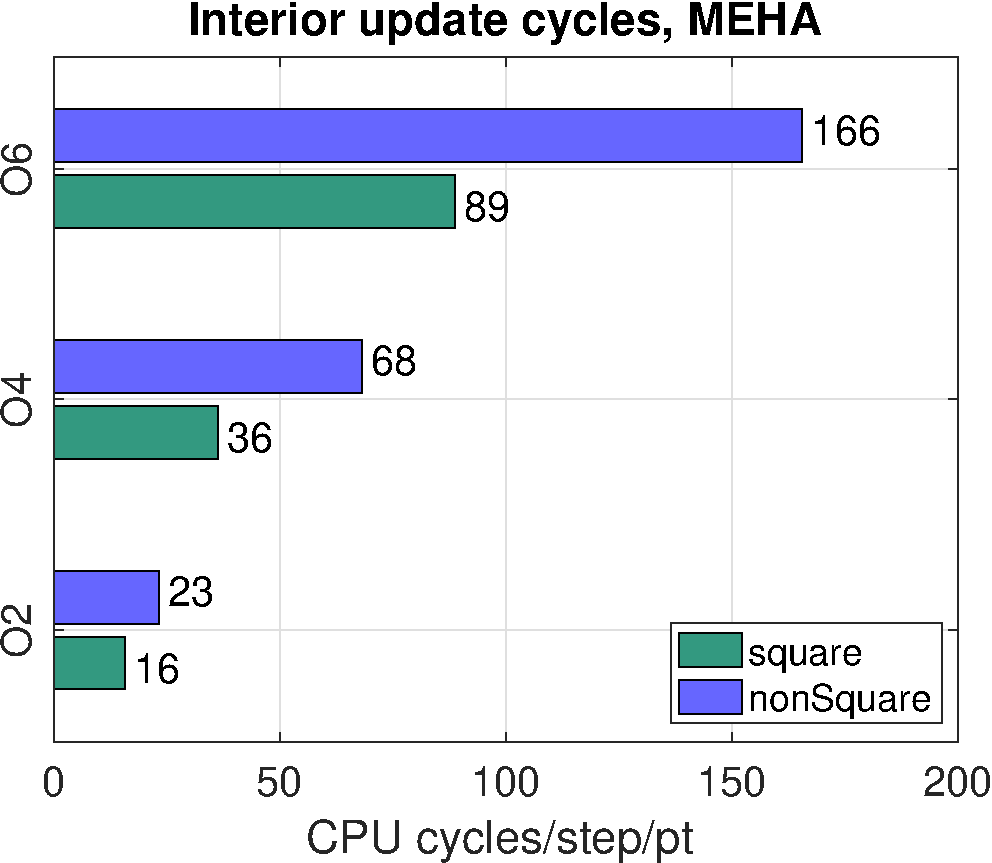
\includegraphics[width=.45\linewidth]{fig/cyclesAdvanceTimesHorizontalBarssquare}
  \quad
  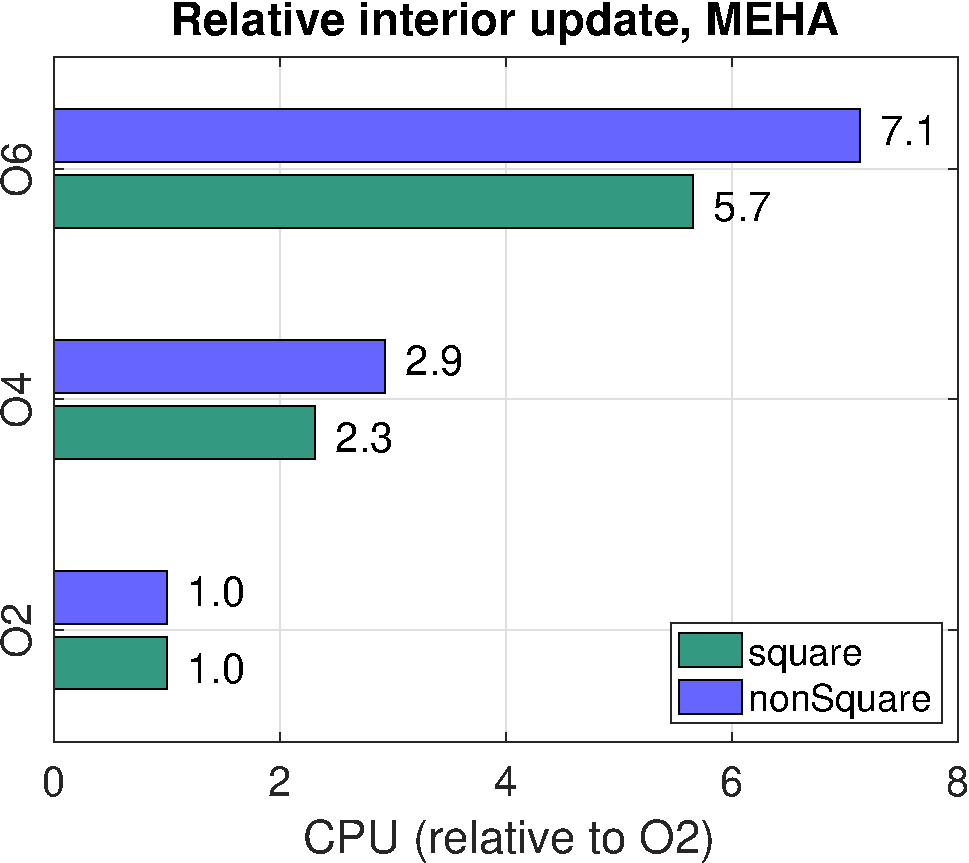
\includegraphics[width=.45\linewidth]{fig/relativeAdvanceTimesHorizontalBarssquare}
  \end{center} 
\caption{Left: CPU cycles per-step per-point (estimates FLOPS per-step per-point). Right: CPU time relative to order 2 scheme.
  Data from Table~\ref{tab:cpuPerformance}.}
\label{fig:relativeSolveTimes}
\end{figure}

\bigskip
Notes for FAME-V2, -O,
\mni
CG6 CPU: 2.7GHz = $2.7\times 10^9 Hz$, clock cycle = $.37\times 10^{-9} = .37$ nano-seconds, (1 nano second = $10^{-9}$ s) 

\mni
% FD22r (Cartesian) has about 9 adds and 7 multiplies : $(9+7) \times .37 ns = 5.9 ns \approx$ CPU for FD22r = $5.8 ns$.
FD22r (Cartesian) has about 8 adds and 7 mults : $15$ FLOPS ($16$ measured)
% (9+7) \times .37 ns = 5.9 ns \approx$ CPU for FD22r = $5.8 ns$.

\mni
FD44r (Cartesian) has about 20 adds and 18 mults : $38$ FLOPS ($36$ measured)
% (20+18) \times .37 ns = 14.1 ns $, FD44r/FD22r = 2.3


\mni
FD22c (curvilinear) has about 16 adds and 10 mults : $26$ FLOPS ($23$ measured)
% $26 \times .37 ns = 9.6 ns$, CPU for FD22c = $13.2 ns$.

\mni
FD44c (curvilinear) has about 47 adds and 30 mults : $77$ FLOPS ($68$ measured)

\mni
FD66c (curvilinear) has about 111 adds and 56 mults : $167$ FLOPS ($166$ measured)

\clearpage
\mni
Test fftw - real 2D transform: 
\begin{Verbatim}[fontsize=\small]
bench -s r1024x1024
Problem: r1024x1024, setup: 275.59 ms, time: 10.19 ms, ``mflops'': 5145.1
Time for 2 FFTs = 2*10.2*10^6/(1024^2)  = 19 ns/pt ->  19/.37 = 51 cycles/pt     log2(N)^2 = 100 

Problem: r1025x1025, setup: 554.93 ms, time: 27.12 ms, ``mflops'': 1937.1
Problem: r1025x1027, setup: 942.77 ms, time: 38.50 ms, ``mflops'': 1367.4
Problem: r1021x1027, setup: 1.34 s, time: 52.31 ms, ``mflops'': 1002.3
Problem: r1223x1223, setup: 2.38 s, time: 128.60 ms, ``mflops'': 596.42

\end{Verbatim}
\begin{Verbatim}[fontsize=\small]
bench -s r2048x2048
Problem: r2048x2048, setup: 534.94 ms, time: 59.32 ms, ``mflops'': 3888.6
Time for 2 FFTs = 2*59.3*10^6/(2048^2) = 28 ns/pt -> 77 cycles/pt
\end{Verbatim}

Test fftw - real 3D transforms
\begin{Verbatim}[fontsize=\small]
bench -s r256x256x256
Problem: r256x256x256, setup: 2.75 s, time: 251.49 ms, ``mflops'': 4002.7
Time for 2 FFTs = 2*251.49*10^6/(256^3) = 30 ns/pt
\end{Verbatim}
\begin{Verbatim}[fontsize=\small]
 bench -s r512x512x512
Problem: r512x512x512, setup: 10.96 s, time: 2.61 s, ``mflops'': 3471
Time for 2 FFTs = 2*2610*10^6/(512^3) = 39 ns/pt
\end{Verbatim}
